%------------------------------------------------------------------------------%
%                                     FDS                                      %
%------------------------------------------------------------------------------%

\section{FDS}

In this section, we will explain what is \gls{fds}, and we will describe some of
the work that has been realized on this tool.

\subsection{The Fire Dynamics Simulator}
\label{sec:fdsdesc}

"\gls{fds} is a computational fluid dynamics (CFD) model of fire-driven fluid
flow. The FDS software solves numerically a form of the Navier-Stokes
nist-equations appropriate for low-speed, thermally-driven flow, with an
emphasis on smoke and heat transport from fires" \cite{fds:pres}. The first
version of the simulator was published in February 2000. It is used for solving
practical problems in fire protection engineering and to studying fundamental
fire dynamics and combustion \cite{fds:tutorial}.

The simulator program reads the configuration from a text file that describe the
parameters, computes the solution of the equations and write the results to
different files. The format of the configuration file is described in the user's
guide \cite{fdsguide}. The output files of the simulator can either be analysed
directly or they can be used as input to other programs. Indeed, \gls{fds} can
be paired with two other programs. Evac is the evacuation simulation module for
\gls{fds}. It is used to simulate the movement of people in evacuation
situations \cite{fds:evac}. Smokeview is a visualization program that displays
the output of \gls{fds}. The figure \ref{fig:smvexample} shows an example of the
Smokeview result. The usage of this tool is described by \cite{smvguide}.

% [Smokeview example] {{{
\begin{figure}[h!]
  \begin{center}
    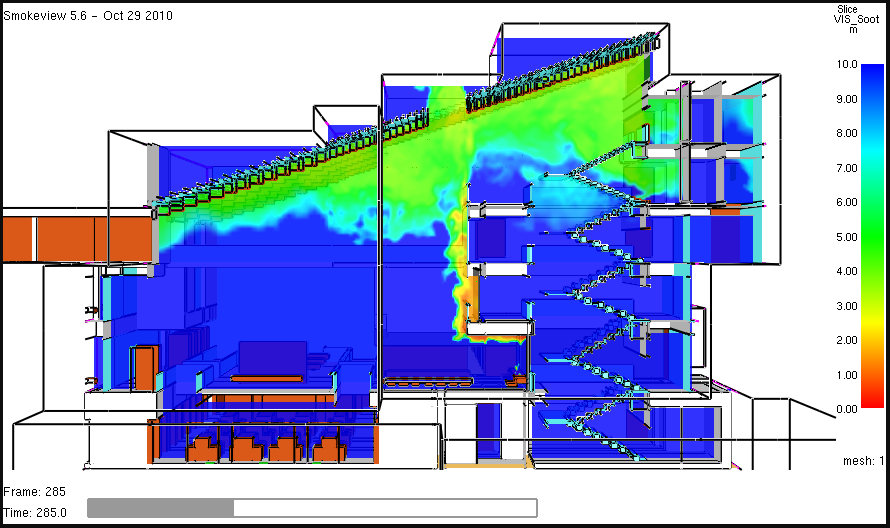
\includegraphics[scale=0.5]{img/smvexample.png}
    \caption{Smokeview example}
    \label{fig:smvexample}
  \end{center}
\end{figure}
%}}}

During the project, neither Evac nor Smokeview have been used. However, it is
still interesting to mention them to give some context.

\gls{fds} uses a large-eddy simulation model (LES) \cite{fdsref}, which is a
mathematical model for turbulence used in computational fluid dynamics
\cite{enwiki:les}. This is an alternative to the direct numerical simulation
(DNS) when the computational costs become too high. The idea is to ignore the
small elements by utilizing a low pass filter on the equations to simplify the
computation \cite{enwiki:les} and \cite{ferziger1996large}. The small elements
can still have an effect on the solution. To solve this problem, \gls{fds}
simulation is divided in two parts as show in the technical reference
\cite{fdsref}. First the predictor part make an estimation of the terms at the
next time step. At the end of the predictor, the simulator verifies the
stability conditions. If the stability conditions are satisfied, the predictor
continues to the next time step. Otherwise, the corrector part will correct the
terms before the simulation continues to the next time step. Both of these steps
will be represented as sub-graphs in the \gls{hh} version of the simulator. The
\gls{fds}'s simulation present many other characteristics that will not be
described in this report. However, all the mathematical tools and models used by
the simulators are detailed by \cite{fdsref}.

The simulation is written entirely in Fortran (standard 2018). The code is
already parallelized using MPI and OpenMP. MPI is used to parallelize the
computation of the meshes \footnote{As explain in the user's guide, a mesh is a
portion of the 3D space. Normally they are used for modeling complex geometrical
structures that do not fit in one parallelogram (corridors for instance).
However, they can also be used to perform a block decomposition on the
matrices.} on multiple nodes on a cluster, and OpenMP is used to parallelize
many of the loops that are present in the program. Interestingly, \gls{fds} do
not use any other dependencies such as \textit{blas} or \textit{lapack} that
we used in the Cholesky implementation. Furthermore, the simulator is not yet
capable of performing GPU computation. However, the developers are interested in
using GPUs in the \gls{hh} implementation.

Now that we have described what \gls{fds} is, let us see what has been done to
optimize the simulation with \gls{hh}.

\subsection{3D loops}

One of the bottleneck of the simulation resides in the computation of the
velocity. This part of the program is composed of three 3D loops that iterates
on the tensors of each mesh, and it can be used several times during a tick of
the simulation. Since it is a critical part of the program, the developers of
\gls{fds} have created a test program, outside the whole simulation, that is
used to measure and try various optimizations. This test program has been very
useful in the effort of optimizing the simulation with \gls{hh} since it was
simple compared to the simulator itself. In this section, we will describe the
test program created by the \gls{fds}'s developers. Then we will explain how the
computation of the velocity has been optimized with the usage of block
decomposition. Finally, we will discuss the limits of the method that has been
used.

\subsubsection{The test program}

As we have seen in the introduction of the section, the test program contains
only the part of the simulation responsible for the computation of the velocity.
The program is composed by three 3D loops parallelized with OpenMP. These loops
are independent, so they are in a parallel section and there are no barriers
between the loops (they run in parallel). The listing \ref{lst:3Dloopscode}
shows the loops with the OpenMP's pragma (all the nested loops are not
represented here).

%- begin listing ------------------------------------------------------------{{{
\begin{listing}[ht!]
\begin{minted}[frame=lines,framesep=2mm,baselinestretch=1.2,fontsize=\normalsize,linenos]{Fortran}
! Compute x-direction flux term FVX

!$OMP PARALLEL PRIVATE(...)
!$OMP DO SCHEDULE(STATIC) PRIVATE(WOMY, VOMZ, TXXP, TXXM, DTXXDX, DTXYDY, DTXZDZ)
DO K=1,KBAR
   ! ...
ENDDO
!$OMP END DO NOWAIT

! Compute y-direction flux term FVY
!$OMP DO SCHEDULE(STATIC) PRIVATE(WOMX, UOMZ, TYYP, TYYM, DTXYDX, DTYYDY, DTYZDZ)
DO K=1,KBAR
   ! ...
ENDDO
!$OMP END DO NOWAIT

! Compute z-direction flux term FVZ
!$OMP DO SCHEDULE(STATIC) PRIVATE(UOMY, VOMX, TZZP, TZZM, DTXZDX, DTYZDY, DTZZDZ)
DO K=0,KBAR
   ! ...
ENDDO
!$OMP END DO NOWAIT
!$OMP END PARALLEL
\end{minted}
\caption{3D loops source code}
\label{lst:3Dloopscode}
\end{listing}
%- end listing --------------------------------------------------------------}}}

The test program is composed in two parts. In the first part, all the variables
are initialized. We will not explain the initialization since it is not present
in the simulator. This initialization is just used to have values on which we
can perform computation. The second part of the program is the computation of
the velocity. We measure the computation time on this part. Finally, the program
computes the mean for each direction (\texttt{FVX}, \texttt{FVY} and
\texttt{FVZ}) in order to have simple values that can be easily verified. The
computation time of the mean is not taken into account when we make the measure
on the original test program unlike on the \gls{hh} program. We will explain why
the \gls{hh} program meausre the computation of the mean as well in the section
\ref{sec:3Dloopsmethod}. Finally, like in the \gls{fds}'s code, most of the
variables are global, which makes difficult to analyse the dependencies between
the tasks.

\subsubsection{The method}
\label{sec:3Dloopsmethod}

To introduce \gls{hh} in this first part of the simulation, the idea was to keep
the entire computation in Fortran. The objective was to be efficient and avoid
rewriting the code in C++. Furthermore, all the variables have been kept in
Fortran as well. Here, \gls{hh} has been used as an orchestrator, its role is to
allocated and managed threads in which the Fortran subroutines are called when
it is required. All the OpenMP's pragmas have been removed since we do not want
to perform fine grain parallelism, we want the threads to be entirely managed by
\gls{hh}.

As we said in the introduction of this section, to optimize computation time, we
have used block decomposition on the 3D arrays of the simulation. In order to do
this, the Fortran code has been reorganized in subroutines that are parametrized
with the boundaries. We can see the declaration of the new subroutines on the
listing \ref{lst:looproutines}. Here we can see as well that we use the ISO C
bindings to be able to call the subroutines from C++. The original loops have
been moved in the new subroutines and have been modified to iterate over the
blocks instead of the whole matrix.

%- begin listing ------------------------------------------------------------{{{
\begin{listing}[ht!]
\begin{minted}[frame=lines,framesep=2mm,baselinestretch=1.2,fontsize=\normalsize,linenos,breaklines=true]{Fortran}
SUBROUTINE COMPUTE_X_FLUX(IBEGIN, JBEGIN, KBEGIN, IEND, JEND, KEND) BIND(C, NAME = "computeXFlux")
SUBROUTINE COMPUTE_Y_FLUX(IBEGIN, JBEGIN, KBEGIN, IEND, JEND, KEND) BIND(C, NAME = "computeYFlux")
SUBROUTINE COMPUTE_Z_FLUX(IBEGIN, JBEGIN, KBEGIN, IEND, JEND, KEND) BIND(C, NAME = "computeZFlux")
\end{minted}
\caption{Loop subroutines signature}
\label{lst:looproutines}
\end{listing}
%- end listing --------------------------------------------------------------}}}

On the listing \ref{lst:loophhtask}, we can see how the subroutines are used in
the \gls{hh} tasks. Here, we can see that the tasks takes as input a block
index. As we have explained, the graph only manages blocks indices. Each block
has the start index and the end index on each dimension. In order to send the
right blocks to the right tasks, the block type as an identifier as template
parameter. This identifier is used to know if the block should be used to
compute the $x$, $y$ or $z$ direction. In the case shown bellow, we want to compute
the terms on the $x$ axis, so the identifier of the block is \texttt{X}.
The same block have been transmitted to the \texttt{Y} and \texttt{Z} tasks
using the corresponding identifiers.

%- begin listing ------------------------------------------------------------{{{
\begin{listing}[ht!]
\begin{minted}[frame=lines,framesep=2mm,baselinestretch=1.2,fontsize=\normalsize,linenos]{C++}
  void execute(std::shared_ptr<BlockIdx<X>> block) override {
    size_t i = block->i == 1 ? 0 : block->i;
    computeXFlux(&i, &block->j, &block->k,
                 &block->iEnd,
                 &block->jEnd,
                 &block->kEnd);
    this->addResult(block);
  }
\end{minted}
\caption{Hedgehog compute task for the 3D Loops program.}
\label{lst:loophhtask}
\end{listing}
%- end listing --------------------------------------------------------------}}}

As we can see on the figure \ref{fig:loopsgraph}, the \gls{hh} graph has three
steps:

\begin{itemize}
  \item Initialization: creation of the blocks indices (has we have seen
    previously, \gls{hh} manages only indices and not the actual data).
  \item Computation of the velocity: this part holds the loops that computes the
    velocity for the x, y and z axis. Here, there is one task per axis, and
    these tasks just call the Fortran subroutines with the blocks boundaries. As
    shown on the graph, all those three tasks are executed in parallel.
  \item Computation of the mean
\end{itemize}

% [3D loops graph] {{{
\begin{figure}[h!]
  \begin{center}
    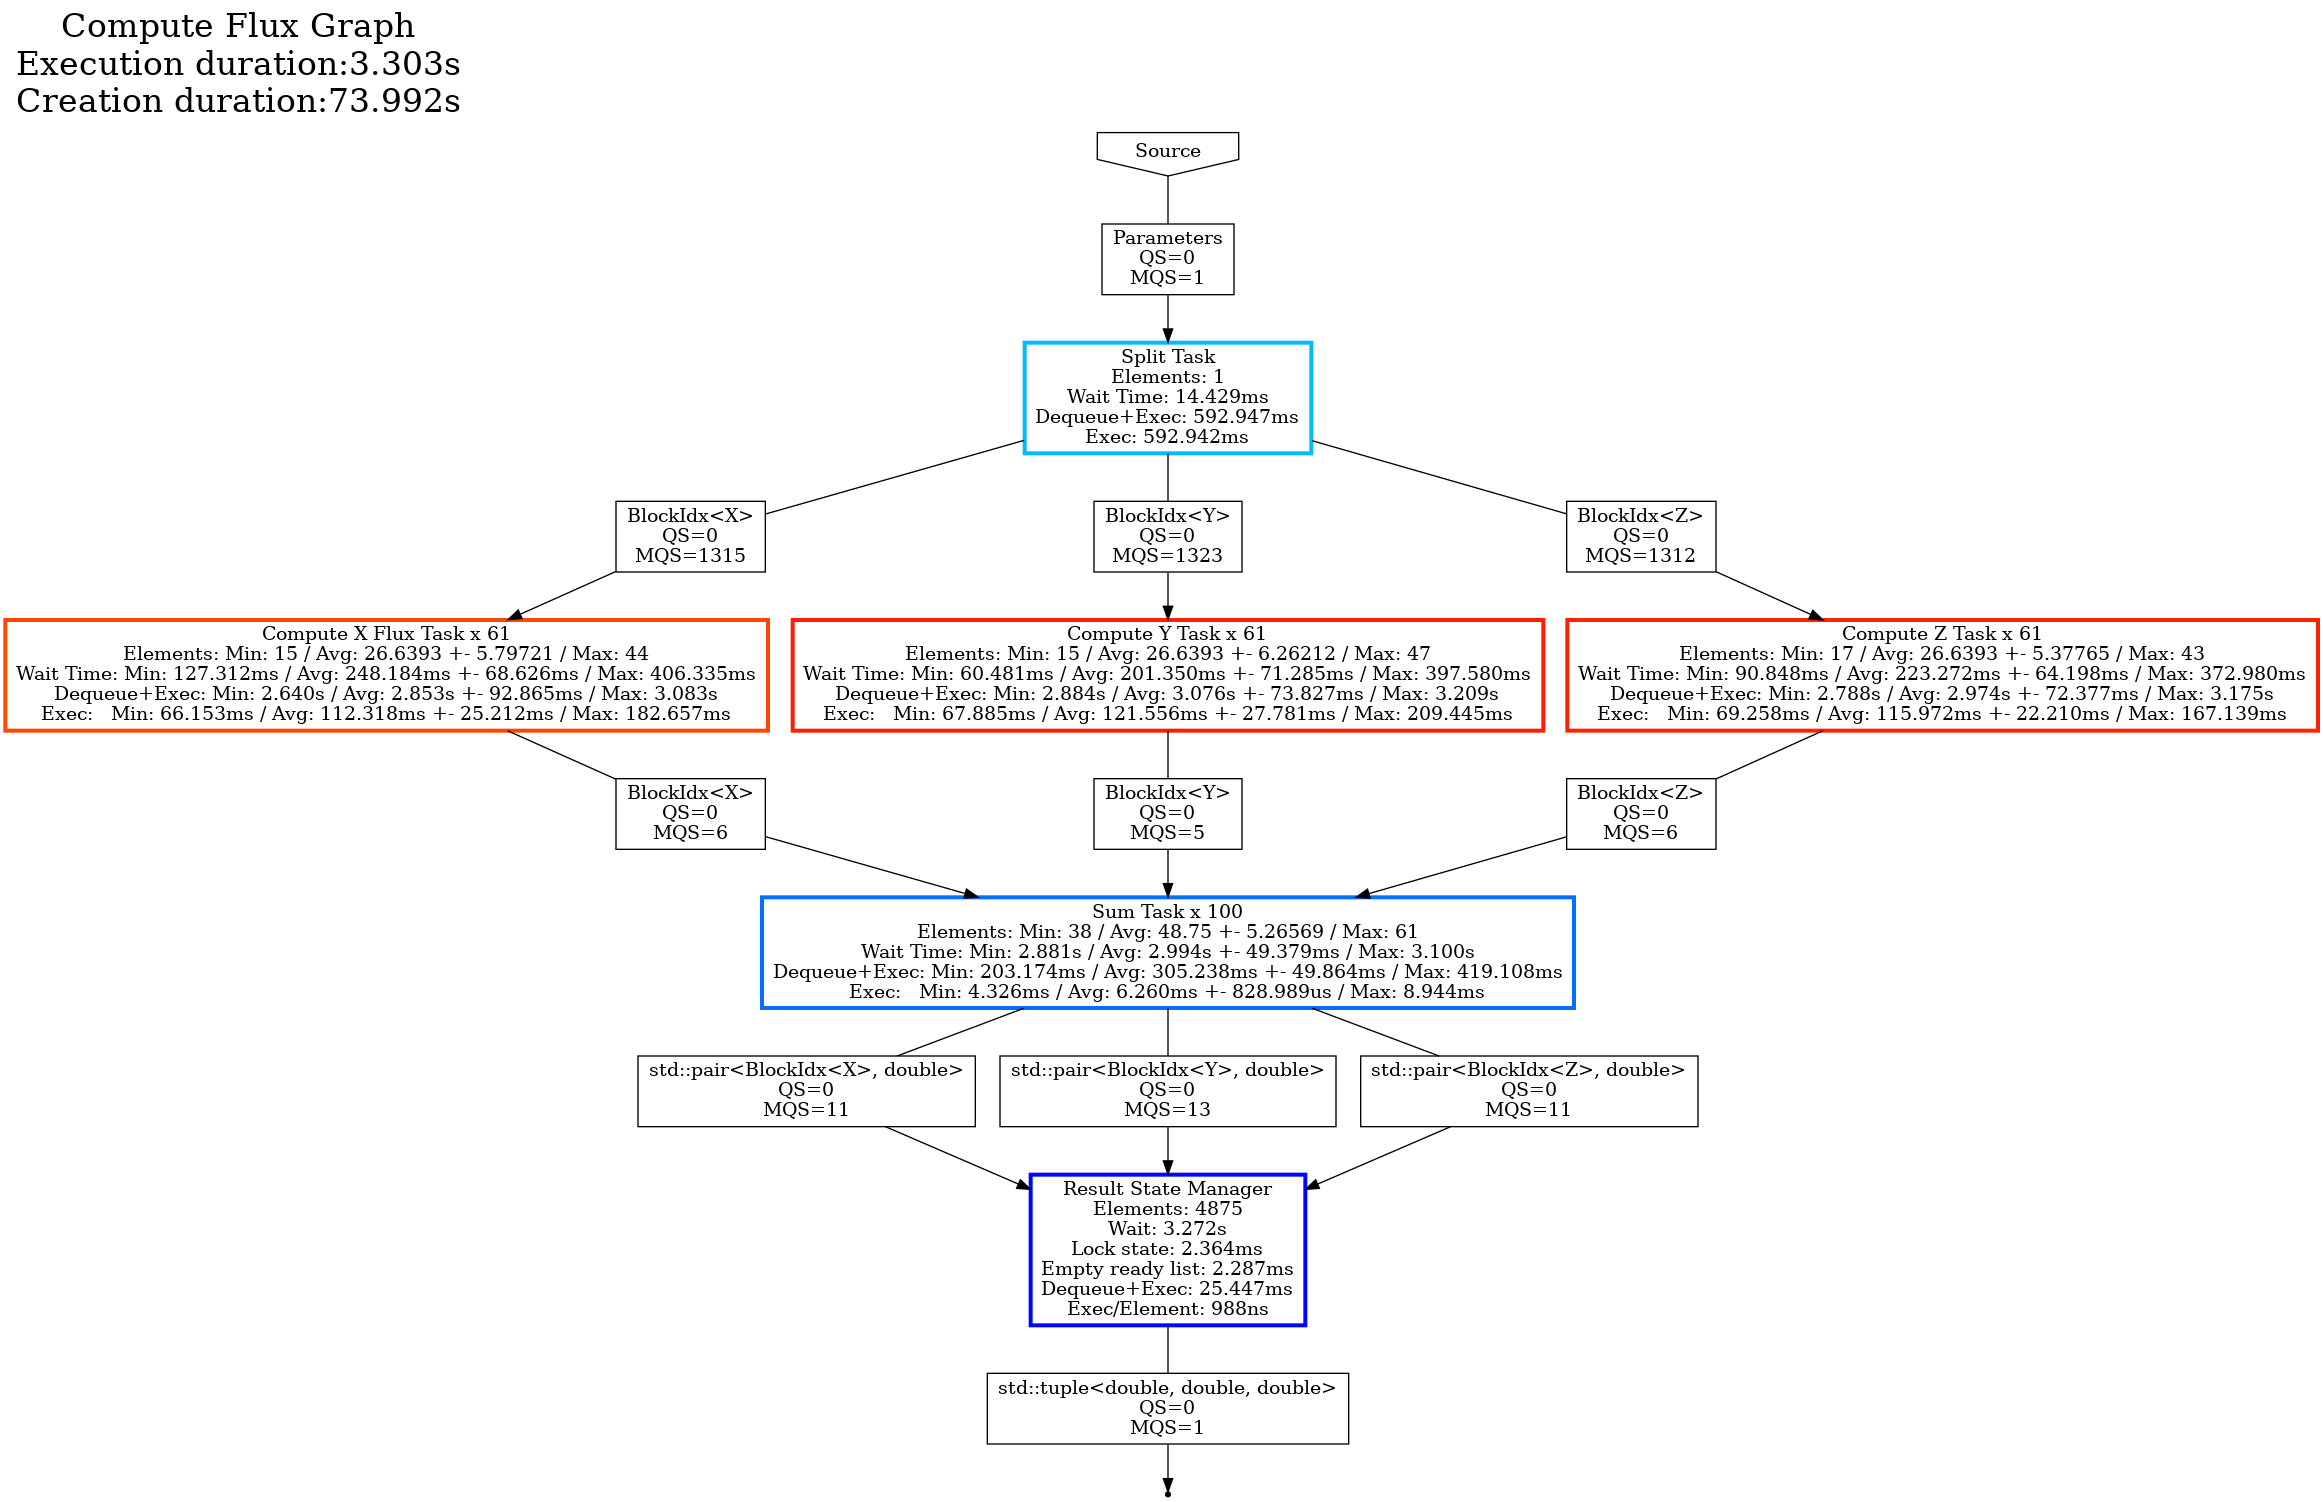
\includegraphics[scale=0.2]{img/fds-loops/graph-61.png}
    \caption{3D loops graph}
    \label{fig:loopsgraph}
  \end{center}
\end{figure}
%}}}

It would have been possible to have only one tasks that perform all the
computation for the three axis. However, having three tasks means that we also
have three queues of data. If we had only one tasks, all the blocks for each
axis would have been in the same queue. To optimize the dequeue time, we use
multiple tasks that run in parallel, and each of these task have its own queue.

\clearpage{}
\subsubsection{The results}

Now that we have explain how the graph has been implemented, we can describe the
results. Before we start, shall we mention that the measure where taken on a
node that has 384 threads, however, here, only 200 threads where available.
Another important detail concern the problem size. In order to test the limits
of the algorithm, the measures have been made on very big matrices
($1024\times1024\times1024$). Though, this is much bigger compared to the size
of the meshes that the algorithm will treat in reality. Making the measures on
such a problem permit to have more distinguishable differences between the
programs, and this allows as well to see if the program scales or not.

Firstly, the plot \ref{fig:loopscomptime} represents the computation of the two
programs. As we can see, the \gls{hh} program is quite faster that the
\gls{fds} one. Furthermore, as shown by the standard deviation, it is way more
consistent. This shows that just by using block decomposition, we are able to
have a faster and more consistent program.

% [Computation times] {{{
\begin{figure}[ht!]
  \begin{center}
    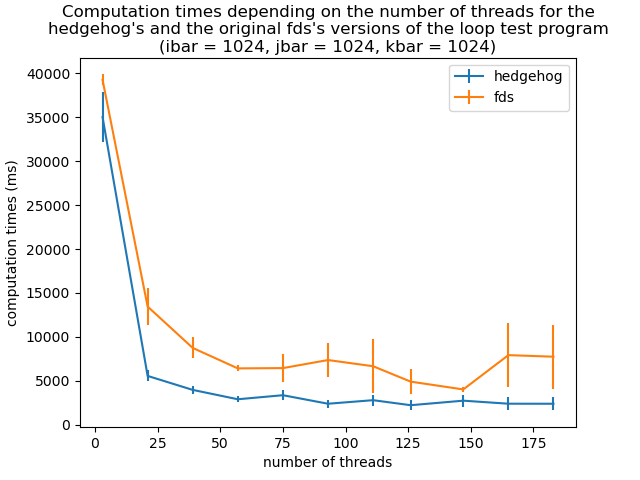
\includegraphics[scale=0.6]{img/fds-loops/times.png}
    \caption{Computation times of the test program for HH and FDS (200 threads node)}
    \label{fig:loopscomptime}
  \end{center}
\end{figure}
%}}}

On the figure \ref{fig:loopsspeedup}, we can see the acceleration of the
\gls{hh} program over the \gls{fds} program. We can notice that on the point
were \gls{fds} has its best measure, \gls{hh} is nearly two times faster.
Interestingly, \gls{fds} starts to be very unstable with more than 150 threads
so the acceleration of the \gls{hh} program is very high.

% [Acceleration] {{{
\begin{figure}[ht!]
  \begin{center}
    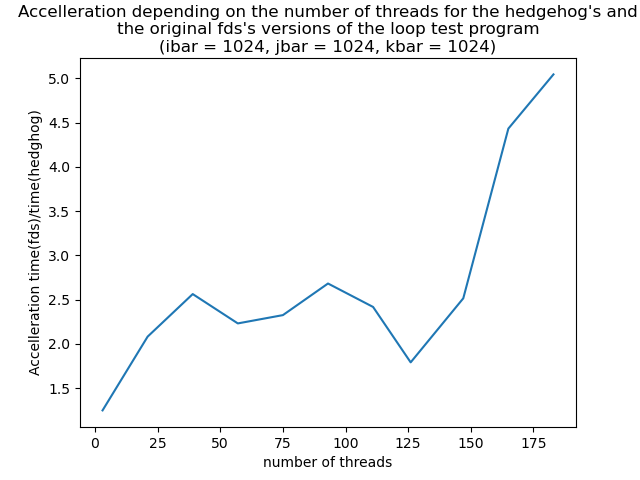
\includegraphics[scale=0.6]{img/fds-loops/speedup.png}
    \caption{Acceleration of HH over FDS on the test program (200 threads node)}
    \label{fig:loopsspeedup}
  \end{center}
\end{figure}
%}}}

Finally, we can see on the figure \ref{fig:loopsrelativespeedup} the relative
speedup for each program. This relative speedup is not very high for both of the
programs which means that we don't reach enough parallelism \footnote{In our
case, having a lot of parallelism means that we use all the resources of the
processors.} yet. For \gls{hh} this can be explained by the fact that the chosen
block size is not optimal. For these measures, the block size was
($1024\times32\times1$), which might be either too large or too small.
Generally, there is no good way to find the optimal block size, the only method
is to test the program with multiple ones. However, this was difficult to do on
this program considering the fact that the initialization is very slow. It took
more than twenty hours of computation to perform the measures that are presented
in this section.

% [Relative speedup] {{{
\begin{figure}[ht!]
  \begin{center}
    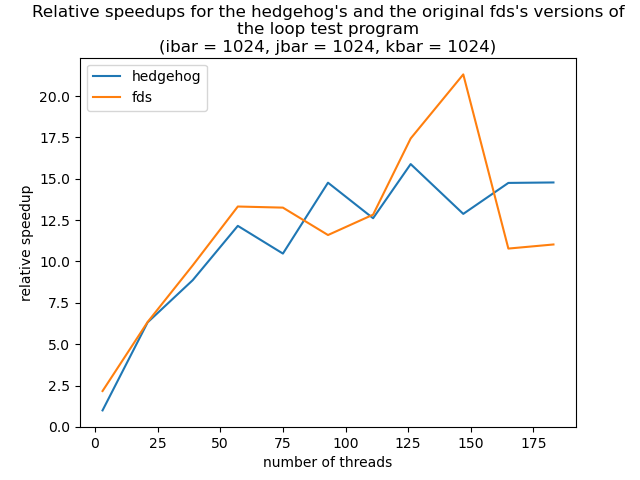
\includegraphics[scale=0.6]{img/fds-loops/relative_speedup.png}
    \caption{Relative speedup for HH and FDS on the test program (200 threads node)}
    \label{fig:loopsrelativespeedup}
  \end{center}
\end{figure}
%}}}

Eventually, these results show that the block decomposition can have a
tremendous impact on the computation time. Furthermore, testing this program
permitted to understand how to use Fortran and C++ together. In the next
section, we will explain why this method can not be used in the global
simulation.

\subsubsection{Limits}

This method works, and it is easy to set up, however it still presents some
limitations.

Firstly, the fact that the data is entirely managed by Fortran is a problem.
Indeed, \gls{hh} creates a data-flow graph, so it should be responsible for
managing all the data. This would have a big impact on the performance, but it
would drastically improve the readability of the graph, as it would allow to
clearly see which task access which data. Having a clear and well organized
graph is very important to keep the application maintainable and expandable.

Secondly, with this method, it is not easy to have computation in C++. Indeed,
have we have seen in the section \ref{sec:cholesky}, some parts of the code have
been entirely rewritten in C++. The fact that we keep all the data as global
variables in Fortran makes nearly impossible to have pure C++ or external
\footnote{Here, external means that the sub-graphs uses other languages.}
sub-graphs. For the data that flows into the global graph, we cannot allow
having them defined in both languages, otherwise, this will require to have
synchronisation tasks in which the data will be copied. Such tasks would have a
tremendous impact on the performance.

Finally, it would not be always possible to keep the types as they currently are
in \gls{fds}. Indeed, as we said in the section \ref{sec:fdsdesc}, the simulator
performs computation on meshes and this computation can be done on multiple
node. Since this meshes belongs to the same geometrical area, after each
computation, we have to synchronise the modifications that have been done on the
stencils \footnote{Area around a mesh that is shared with other meshes} of the
meshes. This is a problem that we will also have with the blocks on the \gls{hh}
version. To perform all the updated efficiently, we will need to have a data
structure that will represent the stencils, and this data structure doesn't
exist in the \gls{fds} code yet. Moreover, we do not want this data structure to
be implemented in Fortran. Firstly because it might be more difficult to
implement (Fortran does not have all the tools that C++ has), and secondly
because the code that will perform the update will be easier to write in C++.

Working on this example program was very useful, primary as it helped to
understand some parts of the code. Furthermore, this was a great demonstration
of what could be done with \gls{hh} on the \gls{fds} code, and it allowed us to
experiment with a part of the code extracted from the whole simulation.
Unfortunately, the method that has been used here cannot be utilized for
parallelizing the rest of the program, but we learned a lot from this exercise.
In the next section, we will discuss the parallelization of the rest of the
simulation.

\subsection{The rest of the simulation}

For now, we have seen the work that has been done on different parts of the
simulation. These part have been treated separately to try different methods for
optimizing the whole code. We have seen that it is possible to rewrite some
sections entirely in C++ like Cholesky. We have tried to use \gls{hh} as an
orchestrator and keep all the computation and the memory in Fortran, and we have
seen why this is eventually not a good idea.

To parallelize the entire simulation with \gls{hh} we have tried to tackle the
problem from two sides. On the first side, the objective was to parallelize
specific pieces of the application, as wee did for the velocity. From the other
side, the idea was to create the general graph and try to set up a pipeline
threw the entire simulation. The role of the global graph is just to call
Fortran subroutines. Our objective from this side is to refactor the graph in
order to have more specific tasks after each iteration. For instance, we start
by having a graph that calls a main function in Fortran. Then we refactor this
graph into a new one that has three tasks: the initialization, the main loop and
the end of the program. Then we try to split each of these three tasks into
sub-tasks to create a new graph, and we keep iterating till our tasks are
precise enough. Eventually, we should end up having atomic tasks, and some of
them can be run in parallel.

This approach was logic, however, it is very difficult to do everything by hand
due to the complexity and the size of the code base. Furthermore, doing this
manually is not a method that is easily reproducible. For this reason, we have
decided to try building a tool able to perform some automatic transformations on
the code.

% todo : reformulate the end and explain why we want to have tool and what it
% does
